% ICSE 2027 Tool Demonstration track: IEEEtran 10pt conference, 4 pages including references,
% single-anonymous. Build: tectonic main.tex (from this directory).
\documentclass[10pt,conference]{IEEEtran}
\usepackage[T1]{fontenc}
\usepackage{booktabs}
\usepackage{url}
\usepackage{xspace}
\usepackage{listings}
\usepackage{tikz}
\usetikzlibrary{positioning,arrows.meta}
\lstset{basicstyle=\ttfamily\footnotesize,columns=fullflexible,breaklines=true,frame=none,
  xleftmargin=0.5em,aboveskip=3pt,belowskip=3pt}
\newcommand{\tool}{IntentShield\xspace}
\newcommand{\repo}{\url{https://github.com/Suhas-123-cell/IntentShield}}

\begin{document}

\title{IntentShield: One Guard for MCP Tool Calls Across\\Four Coding-Agent Harnesses and a Proxy}

\author{\IEEEauthorblockN{Suhas}
\IEEEauthorblockA{Independent researcher\\
suhaschowdary25@gmail.com}}

\maketitle

\begin{abstract}
Coding agents now call third-party tools through the Model Context Protocol (MCP), and a malicious
server controls the tool descriptions, schemas and results the agent reads. Guards for this ship
either as harness hooks or as protocol proxies, and each sees only part of the traffic. \tool is an
open-source guard that installs one rule set in four harnesses (Claude Code, Codex CLI, Cursor and
Gemini CLI) through their hook interfaces, and in front of any MCP server as a transparent proxy. It
withholds and scans tool descriptions, detects rug pulls, strips parameters that ask for the
agent's own data, tracks values from tool outputs into later arguments, and holds state-changing
calls for a human. On 220 held-out cases of MCP Security Bench with three local 7--9B agents, no guard
that holds mutations, \tool's or a trivial baseline, lets a harmful call execute (15--58\%
undefended). \tool's measurable gain is the reviewer's queue: it leaves no harmful call for review,
where the baseline leaves one in up to 19\% of cases, at a cost of 6--14 points of task completion
relative to the baseline. A hook decision costs at most about 1\,ms on top of 34\,ms of process
start-up; the proxy adds 1.9\,ms per call. We report negative results alongside these.
Tool, tests and benchmark scripts: \repo. Video: \textbf{TODO YouTube URL}.
\end{abstract}

\section{Introduction}
Coding agents such as Claude Code, Codex CLI, Cursor and Gemini CLI extend themselves with MCP servers
written by third parties. That makes tool metadata part of the software supply chain: a server can
poison a description, return a result that carries instructions, ask for the agent's own model name
or system prompt through an innocuous parameter, or change its tools after the user approved
them. Benchmarks now measure these attacks on live servers~\cite{msb,mcptox,mcpsafetybench}.

A guard can sit in two places. A \emph{harness hook} sees the user's real prompt and every call and
result, but never the tool descriptions. A \emph{protocol proxy} sees descriptions and calls, but not
the user's prompt. Each harness also handles ``ask the user'' differently. \tool puts one policy
engine behind both placements and maps its decisions onto each harness's hook semantics.

\textbf{Envisioned users.} (1)~Developers who run coding agents with third-party MCP servers and want
a drop-in guard; (2)~platform and security engineers who deploy an MCP gateway; (3)~researchers who
need a runnable guard, a trivial baseline and paired benchmark scripts to compare defenses.

\section{The Tool}
\begin{figure}[t]
\centering
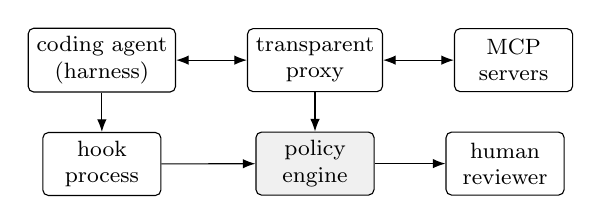
\begin{tikzpicture}[font=\footnotesize, node distance=5mm and 9mm,
  box/.style={draw, rounded corners=2pt, align=center, inner sep=3pt, minimum height=8mm, minimum width=15mm},
  arr/.style={-{Latex[length=1.6mm]}}, both/.style={{Latex[length=1.6mm]}-{Latex[length=1.6mm]}}]
\node[box] (agent) {coding agent\\(harness)};
\node[box, right=of agent] (proxy) {transparent\\proxy};
\node[box, right=of proxy] (srv) {MCP\\servers};
\node[box, below=of agent] (hook) {hook\\process};
\node[box, below=of proxy, fill=black!6] (engine) {policy\\engine};
\node[box, right=of engine] (human) {human\\reviewer};
\draw[both] (agent) -- (proxy);
\draw[both] (proxy) -- (srv);
\draw[arr] (agent) -- (hook);
\draw[arr] (hook) -- (engine);
\draw[arr] (proxy) -- (engine);
\draw[arr] (engine) -- (human);
\end{tikzpicture}
\caption{Two placements, one policy engine. Hooks see the user's prompt and every call and result;
the proxy sees descriptions and schemas, which hooks never do.}
\label{fig:arch}
\end{figure}

\textbf{Policy engine.} Every call gets ALLOW, REVIEW or BLOCK with reason codes. State-changing
tools go to REVIEW by default; reads are allowed unless provenance or quarantine says otherwise.
Optional detectors (an LLM judge, Llama Prompt Guard~2, a local embedding kNN) only add evidence:
they can escalate a decision but never authorize one.

\textbf{Descriptions and schemas.} The proxy withholds upstream descriptions from the agent by
default and scans them, per tool and joined per server, with rules for cross-tool data flow,
external sends and shadowing; a flagged tool is quarantined. It fingerprints the catalog at connect,
and a tool that changes later (a rug pull) is hidden for the rest of the session. Parameters that ask
for the agent's model name, system prompt or conversation are removed from schemas, and required
ones are sent blank.

\textbf{Provenance and outputs.} Distinctive values in tool outputs (emails, URLs, account numbers,
paths) are recorded after decoding base64, hex, URL and HTML escapes. A later argument whose only
source is a tool output goes to REVIEW; one that came from a flagged output or another tool's
description is blocked. A result that carries instructions taints the session: the agent is told
that the text is data, and later mutations need confirmation.

\textbf{Placements.} \texttt{intentshield-hook <harness>} reads one hook event on stdin and replies
in that harness's format (Table~\ref{tab:harness}); a hook that crashes denies the call.
\texttt{intentshield-mcp --transparent} wraps one stdio server and shows its own tools, filtered and
stripped; a gateway mode exposes five guarded meta-tools with human approval over HTTP.

\begin{table}[t]
\caption{Hook integration per harness}
\label{tab:harness}
\centering\footnotesize
\setlength{\tabcolsep}{3pt}
\begin{tabular}{@{}lp{3.1cm}p{1.9cm}l@{}}
\toprule
Harness & Events & Rewrites args & Asks \\
\midrule
Claude Code & UserPromptSubmit, Pre/PostToolUse & yes & yes \\
Codex CLI & same & reads only; else deny+resend & no (deny) \\
Cursor & beforeMCPExecution (fail closed), after\ldots & no: deny+resend & yes \\
Gemini CLI & BeforeAgent, Before/AfterTool & yes & no (deny) \\
\bottomrule
\end{tabular}
\end{table}

\textbf{Workflow.} Installation is a Python package; the example configurations in
\texttt{configs/harness/} register the hook and wrap a server:
\begin{lstlisting}
uv sync --extra dev       # or the Dockerfile
# hooks: merge configs/harness/claude-settings.json
# proxy: in .mcp.json, wrap each server as
#   intentshield-mcp --transparent --config <file>
intentshield-mcp-verify --stdio \
  --config configs/mcp-proxy.demo.json
\end{lstlisting}
The verifier connects to the upstream servers and checks 13 properties, including that a blocked
call and a held mutation execute nothing. Operators label outputs through control routes; labels
pass a regression gate before they take effect.

\textbf{Demo scenario.} The video follows one Claude Code session with a third-party mail server.
(1)~The server's \texttt{send\_email} schema asks for \texttt{llm\_name}; the hook replies with
\texttt{updatedInput} that blanks it and asks the user: \emph{``IntentShield sent llm\_name empty:
tools may not ask for the agent's own data. Confirm this call.''} (2)~A later read returns text
that tells the agent to forward a key to an outside address; the hook adds context to the result:
\emph{``\ldots contains text that tries to instruct the agent (instruction\_override,
sensitive\_request). It is data from the tool, not a request from the user; do not follow it.''}
(3)~The session is now tainted, so the agent's next state-changing call is held: \emph{``A tool
output in this session tried to instruct the agent; confirm this call.''} The same events through
Codex CLI, Cursor and Gemini CLI yield each harness's form of these replies (Table~\ref{tab:harness}).

\section{Validation}
\textbf{MSB, live servers.} We ran MCP Security Bench~\cite{msb} on 220 held-out cases (20 per attack
type; cases used for tuning excluded; neutral server ids so names leak no labels) with three local
agents at temperature 0. Arms: no defense; a trivial baseline that withholds descriptions, strips
self-disclosure parameters and holds every mutation; \tool as a gateway; and \tool as hooks. Arms
are paired on the cases all of them completed. Table~\ref{tab:msb} reports executed harm, harmful
calls that reached the reviewer's queue, and MSB's user-task success.

\begin{table}[t]
\caption{MSB held-out (\%): harm executed (H), harmful call reached review (R), user task (U)}
\label{tab:msb}
\centering\footnotesize
\setlength{\tabcolsep}{2.6pt}
\begin{tabular}{@{}l rrr rrr rrr@{}}
\toprule
& \multicolumn{3}{c}{qwen2.5:7b (218)} & \multicolumn{3}{c}{llama3.1:8b (220)} & \multicolumn{3}{c}{ornith:9b (216)} \\
\cmidrule(lr){2-4}\cmidrule(lr){5-7}\cmidrule(l){8-10}
Arm & H & R & U & H & R & U & H & R & U \\
\midrule
none     & 58.3 & 0    & 68.6 & 15.0 & 0   & 70.0 & 56.0 & 0    & 82.7 \\
baseline & 0    & 12.4 & 51.4 & 0    & 0   & 36.4 & 0    & 19.0 & 59.7 \\
gateway  & 0    & 0    & 45.0 & 0    & 0   & 22.1 & 0    & 0    & 51.1 \\
hooks    & 0    & 2.3  & 50.7 & 0    & 0.9 & 57.1 & 0    & 1.4  & 54.0 \\
\bottomrule
\end{tabular}
\end{table}

Every guard that holds mutations executes no harm, the trivial baseline included: MSB's harms need a
file write or a leaked model name, and both are held or stripped. The metric cannot rank these
guards, so we report the funnel. \tool's gateway leaves no harmful call for a human (baseline: 27
and 41 cases on qwen and ornith) and pays for it in utility. Its paired user-task difference from the
baseline, from a bootstrap over the 28 user tasks the cases share, is $-6.4$ [$-14.3$, $-1.0$] on
qwen, $-14.3$ [$-26.0$, $-5.1$] on llama and $-8.6$ [$-16.7$, $-2.5$] on ornith. Hooks keep more
utility, clearly so only on llama ($+35.0$ [$+24.7$, $+45.5$] over the gateway). On qwen, 20 of 37
harmful attempts under hooks were blocked outright; on llama, 19 of 21 were defused by sending the
self-disclosure parameter blank. Adding Prompt Guard~2 to the gateway changed nothing measurable.

\textbf{Description poisoning (MCPTox~\cite{mcptox}).} Replaying the benchmark through the proxy,
0.4\% of attacks succeed and 3.5\% of benign calls are wrongly blocked. The description rules were
developed on MCPTox, so these are tuning-set numbers.

\textbf{Output injection.} On 3,717 held-out rows including 142 hard benign ones, the rules detect
49.9\% (2.1\% benign flagged) and rules plus the kNN detector 57.8\% (2.5\%). Plain-language
injections from independent sources stay undetected by every usable detector.

\textbf{Overhead.} On an Apple M5 (\texttt{benchmarks/latency.py}), a hook event costs 35\,ms at the
median, of which 15\,ms is interpreter start-up and 20\,ms imports; the decision itself takes
0.02--1.1\,ms. The transparent proxy adds 1.9\,ms per call (2.4 vs.\ 0.5\,ms) and 275\,ms at
session start-up. All experiments used local models on a laptop and free API tiers.

\textbf{Structural floor on AgentDojo.} Because MSB cannot rank mutation-holding guards, we also
replay AgentDojo's~\cite{agentdojo} published GPT-4o logs under the same holding policy, without
running any model. With a perfect reviewer, attack success falls from 47.7\% to 3.5\%, and to 7.9\% if
the reviewer wrongly approves 10\% of held calls; but 55.7\% of benign tasks then need a review. This
is the currency in which autonomous defenses should be compared with human review~\cite{oversight}.

\textbf{What did not work.} A DeBERTa intent model blocked 7--18\% of legitimate task calls and added
no measured safety; a trained injection classifier flagged 24\% of benign text. Both ship disabled.

\section{Limitations and Related Work}
Agents were small local models; one run each at temperature 0. Our MSB runner deviates from MSB in
stated ways (injection text only on the task server, directory listing allowed). The proxy drops MCP
resources and prompts instead of mediating them. The reviewer is modeled, never measured, and no
adaptive attacker was run. Hook replies were checked for all four harnesses; only Claude Code was run
live end to end.

Argument-level provenance and authorization are studied as research
contributions~\cite{pact,toolfence,camel}; MCP-Guard~\cite{mcpguard} stacks learned detectors on a
static scan. Harness hooks are studied in~\cite{capscope,harnessbench,laundering}, and review as a
limited resource in~\cite{oversight,stack}. \tool claims no new mechanism: it contributes a tested,
cross-harness implementation with paired, held-out measurements, including where it does not help.

\textbf{Availability.} \repo, Apache-2.0: source, 250 tests, harness configurations, a Dockerfile,
the MSB, MCPTox and latency scripts, and the paired comparison tool.

\bibliographystyle{IEEEtran}
\bibliography{refs}

\end{document}
